\section{Systembeskrivelse}
Afsnitet systembeskrivelse beskriver de forskellige elektroniske komponenters relation til hinanden via.Til hvert elektriske kredsløb er der et blokdiagram og en uddybende forklaring af blokdiagrammets elementer. Derudover er der et flowdiagram som viser det elektriske kredsløbs funktion.\\

I dette projekt er der i alt 2 forskellige elektriske kredsløb ( hvis man ignorere de isoleret kredsløb, som bliver skabt pga. Brugen af H-broer og hardball pistol). Kredsløb \#1 er kredsløbet som kan findes på selve kanon. Dette kredsløb styrer kanonens bevægelse vha. Motorer og sensorer. Kredsløb \#2 er kredsløbet som findes på kontrolleren. Dette kredsløb bruges til at styrer kanonen gennem et bluetooth signal fra kredsløb \#2 til kredsløb \#1. \\

%Kredsløb 1
\subsection{Kanontårn}

\begin{figure}[H]
\centering
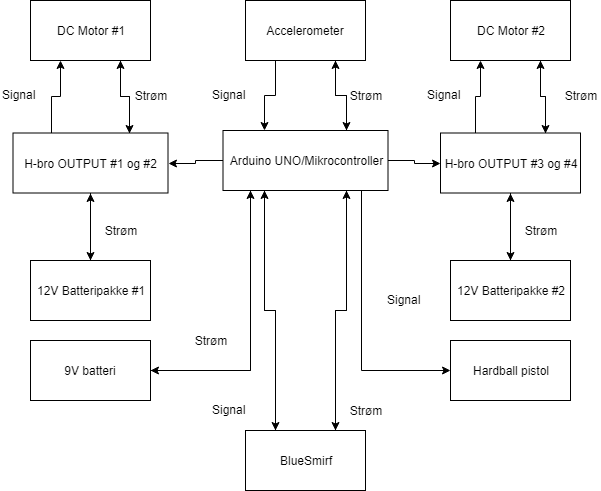
\includegraphics[scale=0.8]{Billeder/Kredsloeb1.png}
\caption{Blokdiagram af kanontaarnets elektriske kredslob.}
\label{fig:Blokdiagram1}
\end{figure}


\begin{figure}[H]
\centering
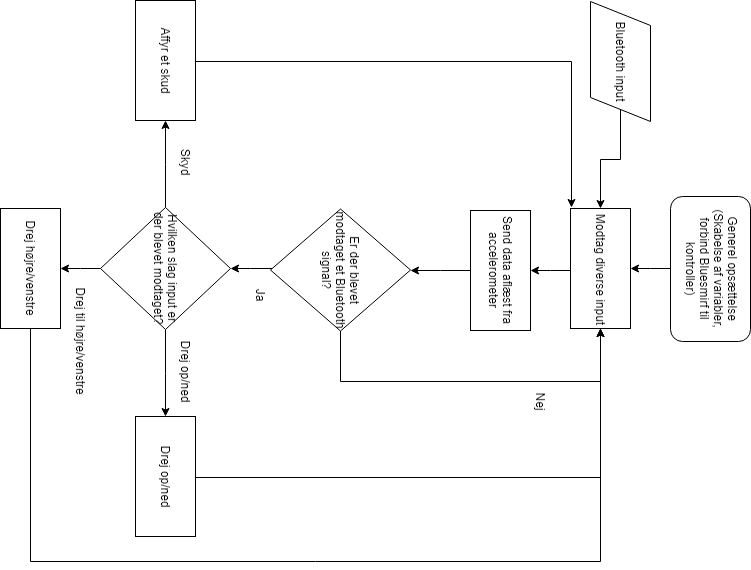
\includegraphics[scale=0.8]{Billeder/Flowchart1.png}
\caption{Flowdiagram af kanontaarnets funktion.}
\label{fig:Flowdiagram1}
\end{figure}

\newpage
\textbf{Systemdele}

%Liste
\begin{itemize}
	\item Arduino UNO / Mikrocontroller
\begin{itemize}
\item På blokdiagrammet kan det ses, at Arduinoen er forbundet til næsten alle elektroniske elementer i kanontårnet. I arduinoens sted kan gruppens egen mikrocontroller print også monteres, da den har samme funktionalitet.
\end{itemize}

	\item 9V batteri
\begin{itemize}
\item Dette 9 volts batteri fungere som Arduinoens / mikrocontrollerens strømforsyning.
\end{itemize}

	\item 6V batteripakke \#1
\begin{itemize}
\item Denne batteripakke fungere som motor \#1’s strømforsyning.
\end{itemize}

	\item 6V batteripakke \#2
\begin{itemize}
\item Denne batteripakke fungere som motor \#2’s strømforsyning.
\end{itemize}

	\item H-bro ( LN298 ) \#1
\begin{itemize}
\item H-bro \#1 er forbundet til motor \#1, 6V batteripakke \#1 og 6V batteripakke \#2. Derudover bliver H-broen kontrolleret af en Arduino, som ikke er i kredsløb med batteripakke \#1 og \#2.
\end{itemize}

	\item Motor \#1
\begin{itemize}
\item Motor \#1 er forbundet til 6V batteripakke \#1 via. H-bro \#1. Derudover er motoren kontrolleret af H-bro \#1. 
\end{itemize}

	\item Stepper Motor \#2
\begin{itemize}
\item Motor \#2 er forbundet til 6V  batteripakke \#2 via. H-bro \#1. Derudover er stepper motoren kontrolleret af H-bro \#1.
\end{itemize}

	\item Accelerometer
\begin{itemize}
\item Accelerometeret er forbundet til Arduinoen, som den desuden også modtager strøm fra.
\end{itemize}

	\item Hardball pistol 
\begin{itemize}
\item Hardball pistolen indgår også i det elektriske kredsløb. Hardball pistolens skyde mekanism bliver kontrolleret af Arduinoen. I selve hardball pistolen findes der også et elektrisk kredsløb, dog er delene til dette kredsløb ikke beskrevet i blokdiagrammet, da det ikke er et selv fabrikeret elektrisk komponent. 	
\end{itemize}

\item BlueSmirf
\begin{itemize}
\item BlueSMiRF komponenten “Silver mate” er forbundet til Arduinoen. BlueSMiRF’en sender og modtager signaler fra Arduinoen. Arduinoen fungerer som strømforsyning til BlueSMiRF’en.

\end{itemize}

\end{itemize}



%Kredsløb 2
\newpage
\subsection{Controller}

\begin{figure}[H]
\centering
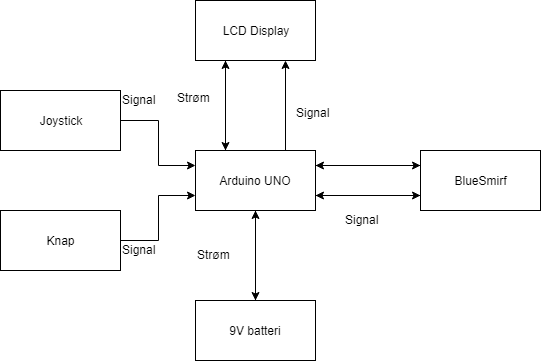
\includegraphics[scale=0.8]{Billeder/Kredsloeb2.png}
\caption{Blokdiagram af controllerens elektriske kredslob.}
\label{fig:Blokdiagram2}
\end{figure}


\begin{figure}[H]
\centering
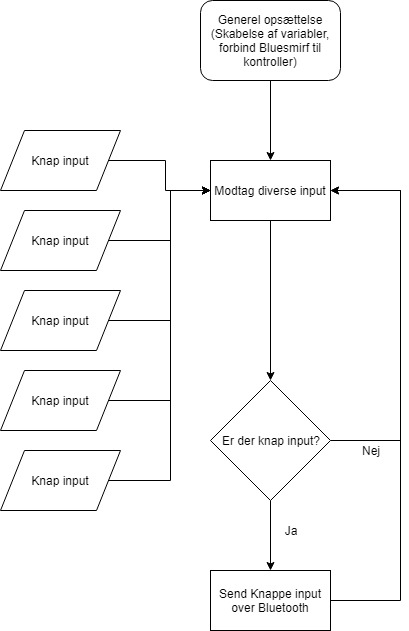
\includegraphics[scale=0.8]{Billeder/Flowchart2.jpg}
\caption{Flowdiagram af controllerens funktion.}
\label{fig:Flowdiagram2}
\end{figure}

\newpage
\textbf{Systemdele}


%Liste
\begin{itemize}
	\item Arduino UNO / Mikrocontroller
\begin{itemize}
\item På blokdiagrammet kan det ses, at Arduinoen er forbundet til næsten alle elektroniske elementer i kanontårnet. I arduinoens sted kan gruppens egen mikrocontroller print også monteres, da den har samme funktionalitet.
\end{itemize}

	\item 9V batteri
\begin{itemize}
\item Dette 9 volts batteri fungere som Arduinoens strømforsyning.
\end{itemize}

	\item Knap \#1
\begin{itemize}
\item Denne knap sender et signal til Arduinoen/Mikrocontrolleren.
\end{itemize}

	\item Knap \#2
\begin{itemize}
\item Denne knap sender et signal til Arduinoen/Mikrocontrolleren.
\end{itemize}

	\item Knap \#3
\begin{itemize}
\item Denne knap sender et signal til Arduinoen/Mikrocontrolleren.
\end{itemize}

	\item Knap \#4
\begin{itemize}
\item Denne knap sender et signal til Arduinoen/Mikrocontrolleren.
\end{itemize}

	\item Knap \#5
\begin{itemize}
\item Denne knap sender et signal til Arduinoen/Mikrocontrolleren.
\end{itemize}

	\item BlueSmirf
\begin{itemize}
\item BlueSMiRF komponenten “Silver mate” er forbundet til Arduinoen. BlueSMiRF’en sender og modtager signaler fra Arduinoen. Arduinoen fungerer som strømforsyning til BlueSMiRF’en.

\end{itemize}


\end{itemize}



